\hypertarget{flexbox}{%
\subsection{Flexbox}\label{flexbox}}

Flexbox, offiziell CSS Flexible Box Layout Module, ist eine neue Art und
ein neues Konzept um eindimensionale Layouts auf Webseiten umzusetzen.
Die herkömmliche Art Objekte auf einer Webseite zu positionieren ist,
fixe Positionen und Maße zu vergeben.

Doch bei Flexbox werden bestimmte Regeln festgelegt, diese machen das
Verhalten der Webseite vorhersagbar bei einer Veränderung der
Bildschirmgröße. Anschließend ist es dem Browser überlassen, die Breite,
Höhe, Position und Anordnung zu wählen.

\hypertarget{das-konzept}{%
\subsubsection{Das Konzept}\label{das-konzept}}

Die Grundidee ist es, dem Flex-Container die Möglichkeit zu geben, die
Maße der Elemente so zu verändern, dass der Platz auf unterschiedlichen
Bildschirmaufslösungen bestmöglich ausgenutzt ist. Um das zu erzielen
lässt das Elternelement die Kindelemente je nach Bedarf wachsen oder
schrumpfen.

\hypertarget{technische-spezifikation}{%
\subsubsection{technische
Spezifikation}\label{technische-spezifikation}}

Innerhalb eines \textless{}div\textgreater{} Tags können die einzelnen
Elemente ihre Größe ``flexibel'' verändern. Sie wachsen, um freien Platz
zu verwenden oder schrumpfen, um innerhalb des Elternobkjekts zu bleiben
und einen Overflow zu vermeiden. Der große Vorteil des Flexbox Layouts
ist die Richtungsunabhängigkeit. Dadurch ist es sehr flexibel, was
Orientierungsänderungen bei mobilen Geräten oder Auflösungsänderungen
auf Desktop Geräten betrifft.

\hypertarget{erkluxe4rung-anhand-eines-realen-beispiels}{%
\subsubsection{Erklärung anhand eines realen
Beispiels}\label{erkluxe4rung-anhand-eines-realen-beispiels}}

Auf dem Dashboard soll eine seitliche Navigation angezeigt werden, die
auf mobilen Geräten an den unteren Rand des Bildschirms wandert, siehe
Abbildung 1.

\begin{figure}
\centering
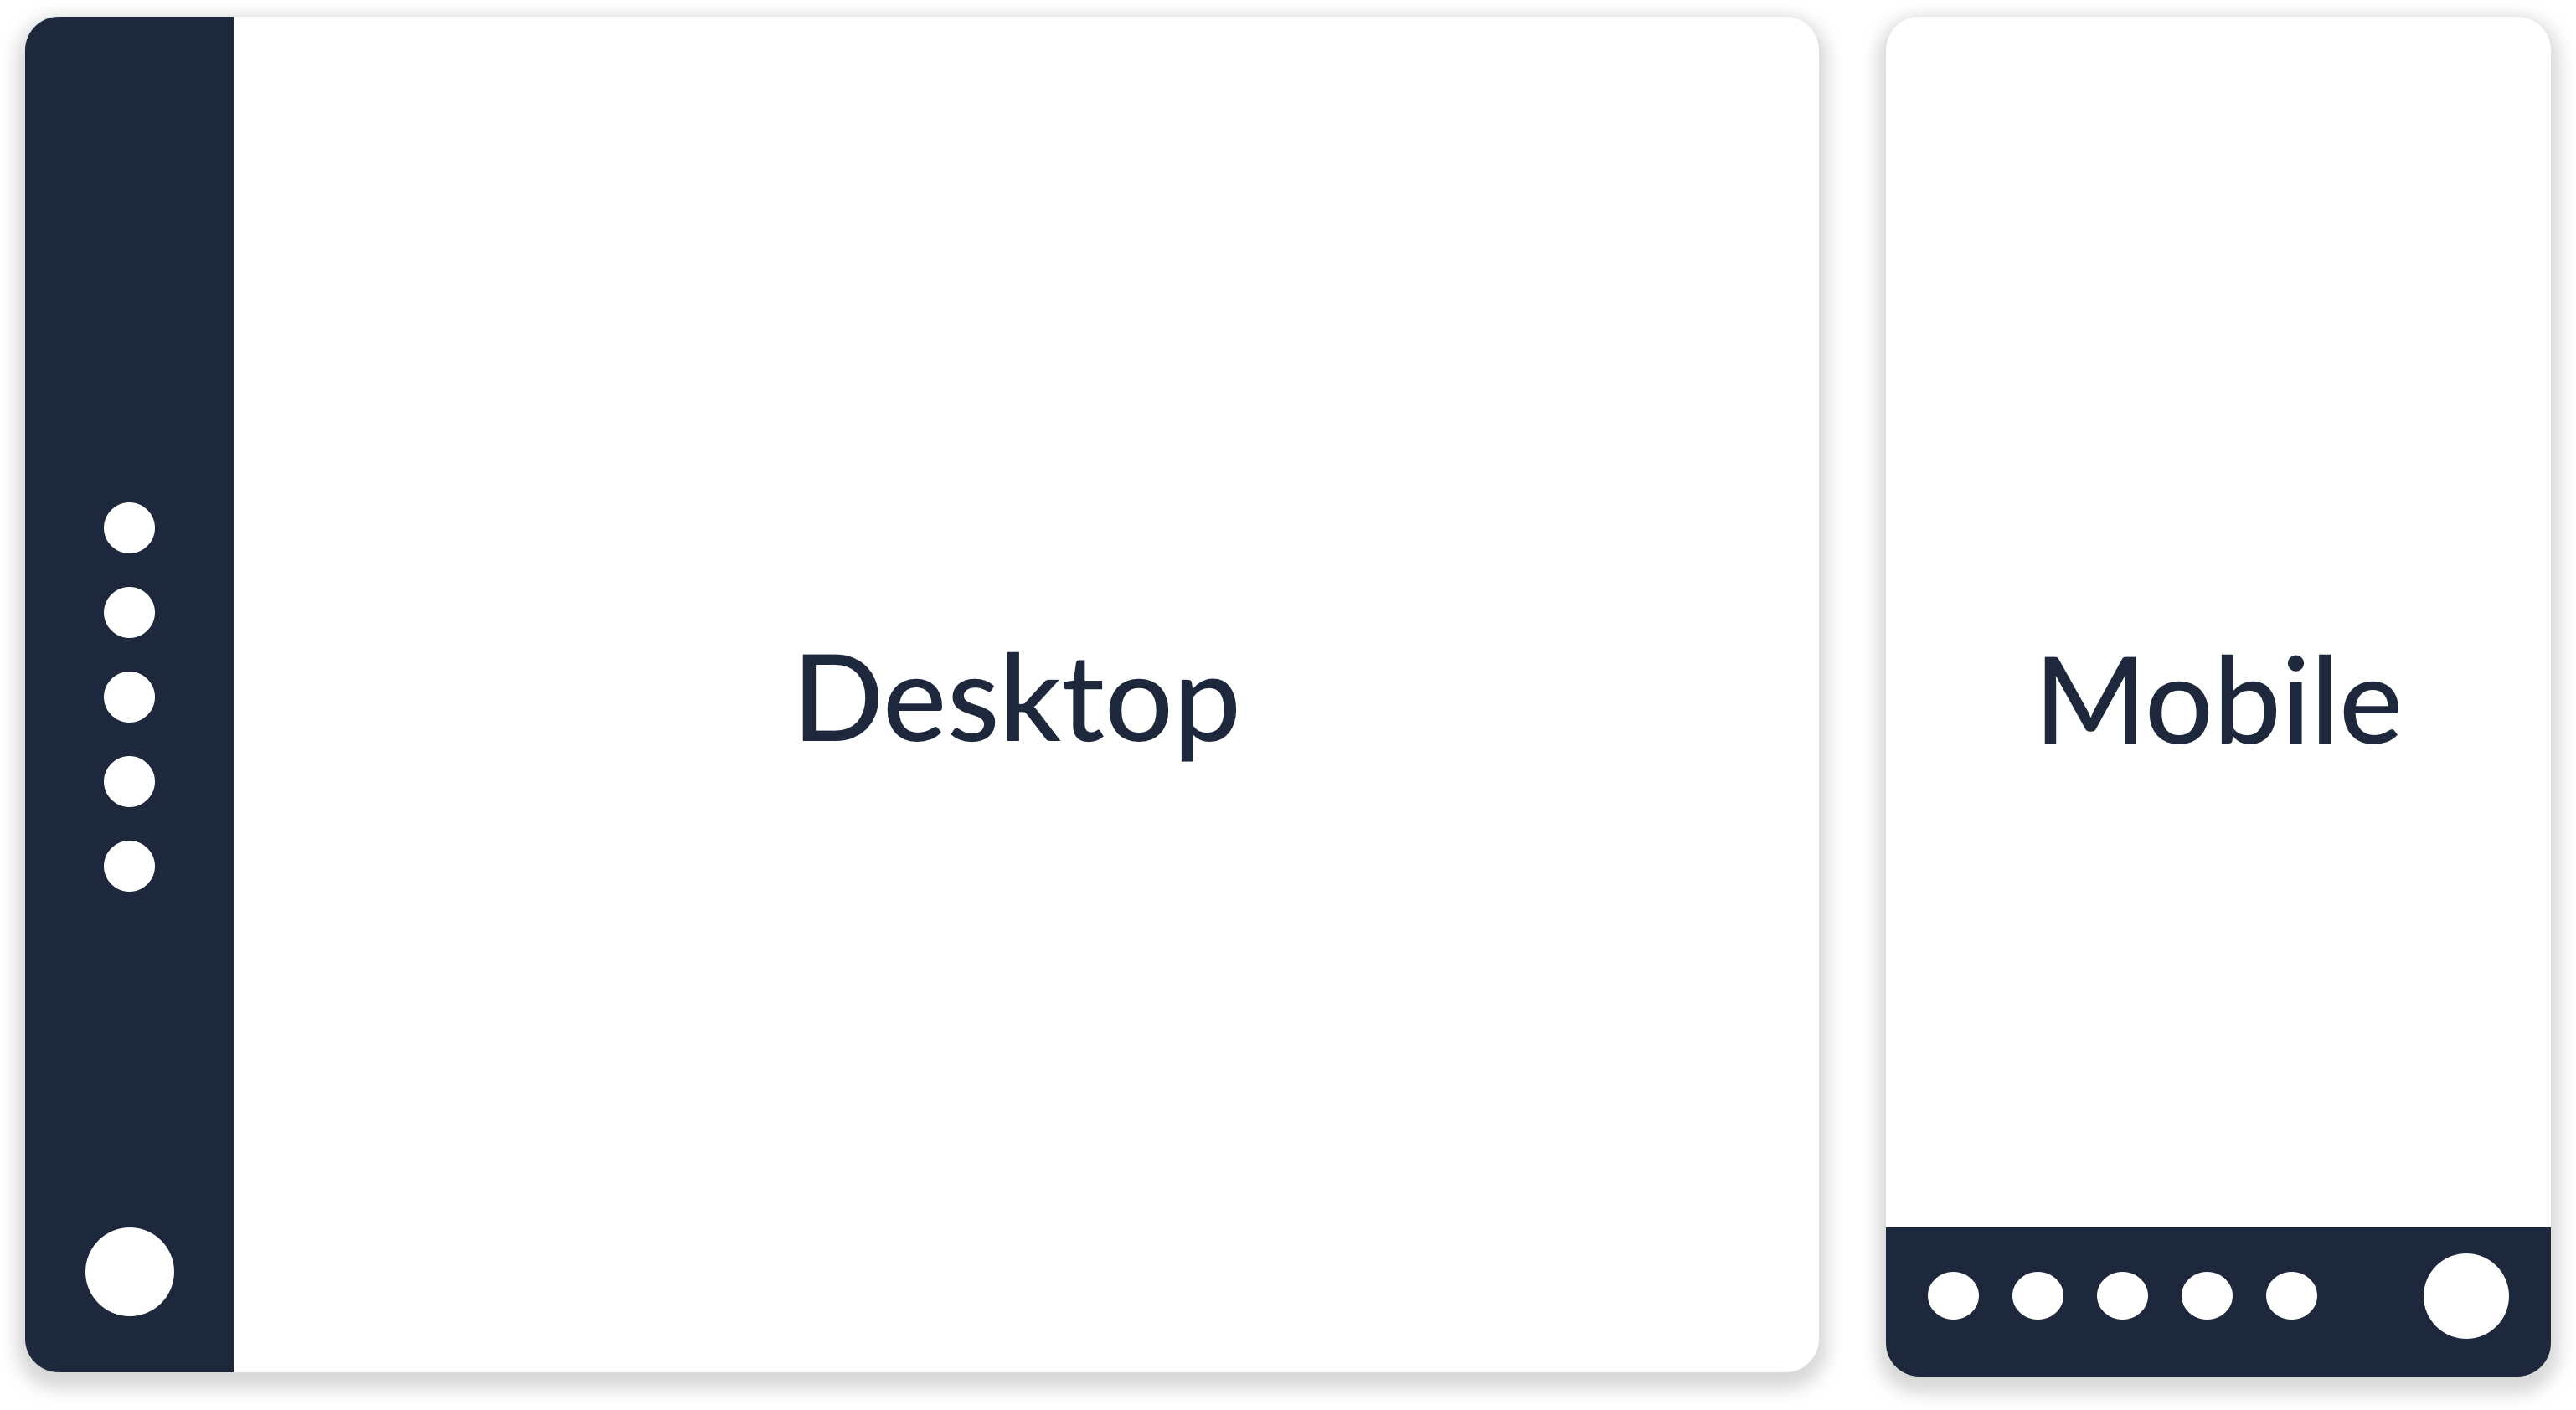
\includegraphics{bilder/Dominik/Flexbox_Illustration_1.png}
\caption{alt text}
\end{figure}

Mithilfe von Flexbox ist dieses Verhalten einfach zu erzielen.\\
Ich erstelle ein Elternelement mit folgenden Eigenschaften:

\begin{Shaded}
\begin{Highlighting}[]
\FunctionTok{.parent}\NormalTok{\{}
  \KeywordTok{display}\NormalTok{: flex;}
  \KeywordTok{overflow}\NormalTok{: }\DecValTok{hidden}\NormalTok{;}
\NormalTok{\}}
\end{Highlighting}
\end{Shaded}

Die Kindelemente dieser Flexbox werden auf der horizontalen Hauptachse
ausgerichtet. Der Overflow auf der X- und Y-Achse wird ausgeblendet. Die
Navigation auf der Seite ist in folgendem Code-Block beschrieben.

Dieses Element ist durch order:1 das erste Element in der Flexbox. Der
Overflow auf der Y-Achse ist versteckt, um die Leiste zu fixieren.
Weiters werden die Elemente innerhalb vertikal und horizontal zentriert
und sind entlang der Y-Achse positioniert.

\begin{Shaded}
\begin{Highlighting}[]
\FunctionTok{.side-nav}\NormalTok{\{}
  \KeywordTok{display}\NormalTok{: flex;}
  \KeywordTok{order}\NormalTok{: }\DecValTok{1}\NormalTok{;}
  \KeywordTok{justify-content}\NormalTok{: }\DecValTok{center}\NormalTok{;}
  \KeywordTok{align-items}\NormalTok{: }\DecValTok{center}\NormalTok{;}
  \KeywordTok{flex-direction}\NormalTok{: column;}
\NormalTok{\}}
\end{Highlighting}
\end{Shaded}

Das Inhaltselement hat order:2 damit es neben dem ersten auf der X-Achse
positioniert wird. Ebenso ist der Overflow auf der Y-Achse versteckt.

\begin{Shaded}
\begin{Highlighting}[]
\FunctionTok{.content}\NormalTok{\{}
  \KeywordTok{overflow-y}\NormalTok{: }\DecValTok{hidden}\NormalTok{;}
  \KeywordTok{display}\NormalTok{: flex;}
  \KeywordTok{justify-content}\NormalTok{: }\DecValTok{center}\NormalTok{;}
  \KeywordTok{flex-direction}\NormalTok{: column;}
  \KeywordTok{order}\NormalTok{: }\DecValTok{2}\NormalTok{;}
\NormalTok{\}}
\end{Highlighting}
\end{Shaded}

Damit die Navigation auf mobilen Geräten am unteren Rand positioniert
ist, benötigen wir eine Media Query. Mithilfe dieser können CSS-Stile
anhand von verschiedenen Eigenschaften wie z.B. Bildschirmauflösung oder
Seitenverhältnis manipuliert werden. Im untenstehenden Code-Block wird
dies veranschaulicht. Indem wir die Hauptachse des Flexbox
Elternelements auf die Y-Achse ändern, werden die beiden Kindelemente
nun vertikal verteilt. Damit nun auch die Navigation unter dem Inhalt
positioniert ist ändern wir die order auf 2. Weiters müssen die Höhe und
Breite angepasst werden.

\begin{Shaded}
\begin{Highlighting}[]
\ImportTok{@media}\NormalTok{ (}\KeywordTok{max-width}\NormalTok{: }\DecValTok{576px}\NormalTok{)\{}
  \FunctionTok{.parent}\NormalTok{\{}
    \KeywordTok{flex-direction}\NormalTok{: column; //changed}
\NormalTok{  \}}

  \FunctionTok{.side-nav}\NormalTok{\{}
      \KeywordTok{order}\NormalTok{: }\DecValTok{2}\NormalTok{;             //changed}
      \KeywordTok{width}\NormalTok{: }\DecValTok{100vw}\NormalTok{;         //changed}
      \KeywordTok{height}\NormalTok{: }\DecValTok{66px}\NormalTok{;         //changed}
\NormalTok{    \}}
\NormalTok{  \}}
\end{Highlighting}
\end{Shaded}

